%Verification techinques:
%\begin{itemize}
%\item Safety Verification
%\item Performance analysis	
%\end{itemize}
%A \textit{safety} property is intuitively defined in the formal verification context as a property stating that something ``bad'' will \textit{never} happen during execution.\cite{lamport1}
%Cassical examples of safety properties are deadlock freedom and mutual exclusion, where the ``bad'' behaviour is respectively the deadlock occurrence and the simultaneous execution of a critical section.
%One of the most important requirements for streaming systems is guaranteeing low latency while maintaining high throughput. 
%In a distributed  --> Motivare questione delle code!
%

%
%\subsection{Storm Formal Model}
%\label{sec:storm-model}
%To perform our verification tasks we defined a formal model expressed in CLTLoc with discrete variables. The resulting model is a non-deterministic infinite state system.

% MOVED BEFORE
%%%\subsubsection{OSTIA Models: a Formal Interpretation}
%%%We started by understanding and capturing the behaviors of both spouts and bolts. 
%%%After choosing the level of abstraction of our model we simplified those behaviors accordingly, in order to formalize them as finite state machines. The purpose of this first activity was to define the possible operations and the allowed orderings of such operations.
%%%We then extended the model by taking into account the message buffers (or queues) and the quantity of tuples that are exchanged through the topology.
%%%In addition to the correct ordering of the operations, we decided to introduce more specific temporal constraints into the model, in order to limit the time spent by the system in each state (or processing phase) and to elaborate the concept of \textit{rate}, intended as ``number of times an event is occurring every time unit''.\\

%\subsubsection{Assumptions and  level of abstraction}
%We made several assumptions and abstractions while building the model:

Building on top of the above framework,  a formal interpretation of the Storm (meta-)model requires several abstractions and assumptions.

%For example, some deployment details, such as the number of worker nodes and features of the underlying cluster, are abstracted away. 
%There is a single queuing layer: every bolt has a unique incoming queue and no sending queue, while the worker queues are not represented. In the same way, each bolt/spout has a single output stream.
%Moreover, the content of messages is not relevant: all the tuples have the same fixed size and we represent only quantity of tuples moving through the system.


\begin{itemize}
	\item some deployment details, e.g., the number of worker nodes and features of the underlying cluster, are abstracted away;
	\item each bolt/spout has a single output stream;
	\item %we simplified the message buffer system, assuming that 
	there is a single queuing layer: every bolt has a unique incoming queue and no sending queue, while the worker queues are not represented;
	\item every operation is performed within minimum and maximum thresholds of time;
	\item %we do not take into account 
	the content of the messages is not relevant: all the tuples have the same fixed size and we represent only quantity of tuples moving through the system;
\end{itemize}

%\subsubsection{Model Formalization}
A Storm Topology is a directed graph $\mathbf{G} = \{ \mathbf{N}, Sub\}$ where the set of nodes $\mathbf{N} = \mathbf{S}\bigcup \mathbf{B}$ includes in the sets of spouts (\textbf{S}) and bolts (\textbf{B}) and %the set of edges $\mathbf{E} = \{ Sub_{i,j} | i \in \mathbf{B}, j \in \{\mathbf{S}\bigcup \mathbf{B}\} \}$ 
$Sub\subset\mathbf{N}\times\mathbf{N}$ defines how the nodes are connected each other via the subscription relation. Pair $(i,j)\in Sub$ indicates that ``bolt $i$ subscribes to the streams emitted by the spout/bolt $j$''. 
Spouts cannot subscribe to other nodes in the topology.
Each bolt has a receive queue where the incoming tuples are collected before being read and processed. % by the node.
The queues have infinite size and the level of occupation of each $j^{th}$ queue is described by the variable $q_j$. %\footnote{Spouts have no queues, by definition.}
Spouts have no queues, and 
each spout can either \textit{emit} tuples into the topology or stay \emph{idle}.
Each bolt can be in \emph{idle} state, in \emph{failure} state or in  \emph{processing} state.  While in the processing state, the bolt first reads tuples from its receive queue (\textit{take} action), then it performs its transformation (\textit{execute} action) and finally it \textit{emits} the output tuples in its output streams. \\
\begin{figure}[tb]
\centering
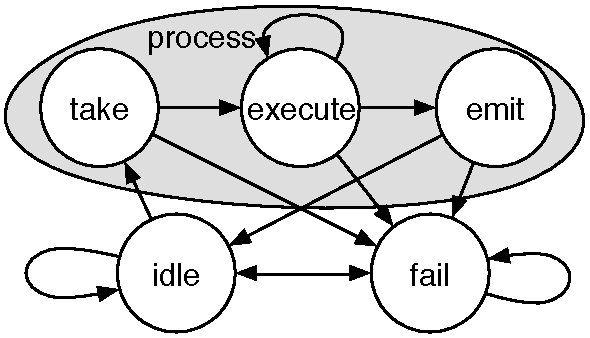
\includegraphics[width=0.7\linewidth]{images/bolt-fsm}
\caption{Finite state automaton describing bolt states.}
\label{figure-fsa}
\end{figure}

%\begin{figure}
%	\centering	
%	\begin{tikzpicture}[->,>=stealth',shorten >=1pt,auto,node distance=2.5cm,semithick, every node/.style={scale=0.55}]
%	
%	\tikzstyle{every state}=[fill=white,text=black,minimum width={width("execute")+10pt}]
%	
%	
%	\node[state]            (I) {$idle$};  
%	\node[state]         (T) [above right of=I] {$take$};  
%	\node[state]         (E) [right of=T] {$execute$};
%	\node[state]         (F) [below right of=I] {$fail$};
%	\node[state]         (EM) [right of=F] {$emit$};
%	
%	\path (I) edge              node {} (T)
%	edge              node {} (F)
%	edge [loop above]  node {} (I)
%	(E) edge [loop right] node {} (E)
%	edge              node {} (EM)
%	(T) edge              node {} (E)
%	edge              node {} (F)
%	(EM) edge             node {} (I)
%	edge              node {} (F)
%	(F) edge [loop below]  node {} (F);
%	edge [bend right]  node {} (I);
%	\end{tikzpicture}
%	\caption{Finite state automaton describing bolt states.}
%	\label{figure-fsa}
%\end{figure}
%To give an idea about how the model is formalized, 
We provide, as an example, one of the formulae defining the processing state. Formula \ref{formula:1} can be read as \textit{``for all bolts: if a bolt j is processing tuples, then it has been processing tuples since it took those tuples from the queue, (or since the origin of the events), and it will keep processing those tuples until it will either emit them or fail. Moreover, the bolt is not in a failure state''.}
\begin{align}
\small
%
\bigwedge_{
	i \in \mathbf{B} } 
\left( 
\begin{array}{l}
\p{i} \Rightarrow \\
\p{i} \, \Snc \, ( \ta{i} \lor (\ori \land \p{i})) \land \\
\p{i} \, \U \, (\e{i} \lor \f{i}) \land \lnot \f{i} 
\end{array}
\right) \label{formula:1} 
%
\end{align}
The number of tuples emitted by a bolt depends on the number of incoming tuples. The ratio $\frac{\#output\_tuples}{\#input\_tuples}$ %is used to 
expresses the ``kind of function''  performed by the bolt and is given as configuration parameter. 
All the emitted tuples are then added to the receive queues of the bolts subscribing to the emitting nodes.
In the same way, whenever a bolt reads tuples from the queue, the number of elements in queue decreases. To this end, formula \ref{formula:2}, imposes that \textit{``if a bolt takes elements from its queue, the number of queued elements in the next time instant will be equal to the current number of elements plus the quantity of tuples being added (emitted) from other connectd nodes minus the quantity of tuples being read''.}
\begin{align}\small
%
\bigwedge_{
	\begin{subarray}{c}
	\,j \in B
	\end{subarray}
} &( \ta{j}{}  \Rightarrow (\aX q_j = q_j + \ra{j} - \rt{j} )) \label{formula:2}
%
\end{align}
These functional constraints are fixed for all the nodes and they are not configurable.
%What is configurable and can be tuned changing the parameters of the model is everything concerning 
The structure of the topology, the parallelism level of each node, the bolt function and the non-functional requirements, as, for example, the time needed for a bolt in order to process a tuple, the minimum and maximum time between failures and the spout emitting rate are configurable parameters of the model.
Currently, the verification tool accepts %as configuration format 
a JSON file containing all the configuration parameters.
OSTIA supports such format and is able to extract from static code analysis a partial set of features, and an almost complete set of parameters after monitoring a short run of the system. The user can complete the JSON file by adding some verification-specific settings.


